\chapter{Teoretická část}
\section{Suspendace}
Smyslem suspendace v mechanicky míchaných nádobách je udržení pevných částic ve vznosu tak, aby došlo ke zintenzivnění transportu hmoty a tepla mezi kapalinou a pevnou fází. Pro dosažení tohoto stavu je třeba systému dodat energii v podobě mechanické práce. K vykonání této práce se používají rozmanité typy mechanických míchadel, které jsou voleny podle konkretního charakteru dané úlohy. Dodaná energie poté vede k vytvoření turbulentního proudění, jenž uvede částice pevné fáze do vznosu a následně je rozptýlí v kapalině. Nutnou podmínkou pro zajištění tohoto vznosu je potřeba, aby výsledná vertikální složka síly působící na částici byla větší než tíhová síla zmenšená o sílu vztlakovou. Menší částice jejichž hustota je přibližně rovna hustotě kapalina se po dosažení suspenzních podmínek pohybují společně s kapalinou. Při nižších koncentracích pevné fáze se toto proudění chová spíše jako jednofázový tok. Naopak rychlost pohybu těžších částic se liší od rychlosti kapalné fáze, jenž musí na pevnou fázi působit větší silou k zabránění jejímu usazování. Výslednou kvalitu vzniklé suspenze ovlivňuje řada faktorů, kde mezi nejvýznamnější patří fyzikální vlastnosti, jak kapalné, tak pevné fáze, provozní podmínky a geometrie systému a míchadla.

\subsection{Stupně suspendace}


\begin{figure}[h!]
  \centering
  \subfloat[Částečná]{\label{fig:typ1}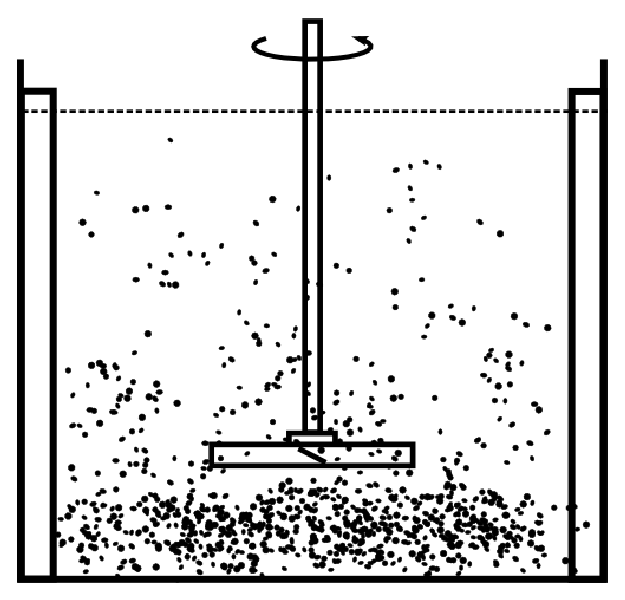
\includegraphics[scale=0.35]{images/typy_suspenzi-1.eps}}
  \qquad
  \subfloat[Úplná]{\label{fig:typ2}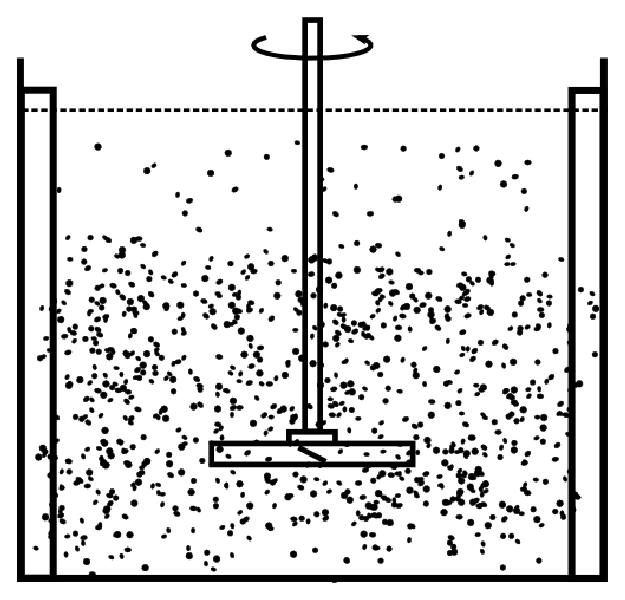
\includegraphics[scale=0.35]{images/typy_suspenzi-2.eps}}
  \qquad
  \subfloat[Homogenní]{\label{fig:typ3}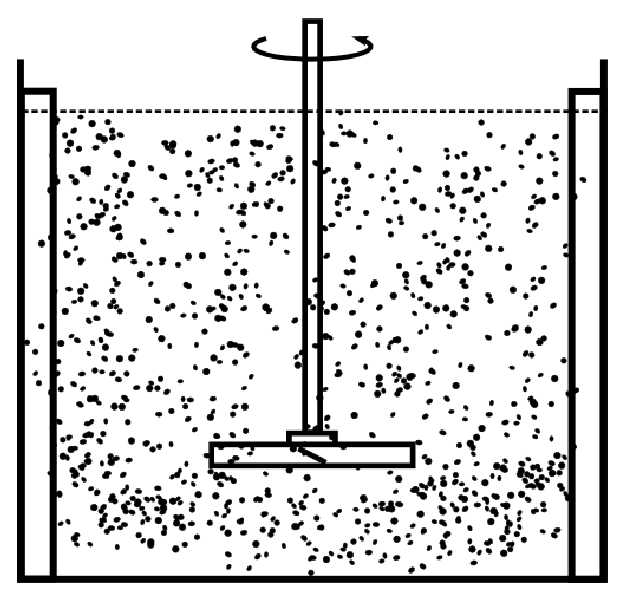
\includegraphics[scale=0.35]{images/typy_suspenzi-3.eps}}
  \caption{Stupně suspendace}
  \label{fig:typsus}
\end{figure}




\section{Počítačová dynamika tekutin (CFD)}



